% Template for PLoS
% Version 3.5 March 2018
%
% % % % % % % % % % % % % % % % % % % % % %
%
% -- IMPORTANT NOTE
%
% This template contains comments intended
% to minimize problems and delays during our production
% process. Please follow the template instructions
% whenever possible.
%
% % % % % % % % % % % % % % % % % % % % % % %
%
% Once your paper is accepted for publication,
% PLEASE REMOVE ALL TRACKED CHANGES in this file
% and leave only the final text of your manuscript.
% PLOS recommends the use of latexdiff to track changes during review, as this will help to maintain a clean tex file.
% Visit https://www.ctan.org/pkg/latexdiff?lang=en for info or contact us at latex@plos.org.
%
%
% There are no restrictions on package use within the LaTeX files except that
% no packages listed in the template may be deleted.
%
% Please do not include colors or graphics in the text.
%
% The manuscript LaTeX source should be contained within a single file (do not use \input, \externaldocument, or similar commands).
%
% % % % % % % % % % % % % % % % % % % % % % %
%
% -- FIGURES AND TABLES
%
% Please include tables/figure captions directly after the paragraph where they are first cited in the text.
%
% DO NOT INCLUDE GRAPHICS IN YOUR MANUSCRIPT
% - Figures should be uploaded separately from your manuscript file.
% - Figures generated using LaTeX should be extracted and removed from the PDF before submission.
% - Figures containing multiple panels/subfigures must be combined into one image file before submission.
% For figure citations, please use "Fig" instead of "Figure".
% See http://journals.plos.org/plosone/s/figures for PLOS figure guidelines.
%
% Tables should be cell-based and may not contain:
% - spacing/line breaks within cells to alter layout or alignment
% - do not nest tabular environments (no tabular environments within tabular environments)
% - no graphics or colored text (cell background color/shading OK)
% See http://journals.plos.org/plosone/s/tables for table guidelines.
%
% For tables that exceed the width of the text column, use the adjustwidth environment as illustrated in the example table in text below.
%
% % % % % % % % % % % % % % % % % % % % % % % %
%
% -- EQUATIONS, MATH SYMBOLS, SUBSCRIPTS, AND SUPERSCRIPTS
%
% IMPORTANT
% Below are a few tips to help format your equations and other special characters according to our specifications. For more tips to help reduce the possibility of formatting errors during conversion, please see our LaTeX guidelines at http://journals.plos.org/plosone/s/latex
%
% For inline equations, please be sure to include all portions of an equation in the math environment.
%
% Do not include text that is not math in the math environment.
%
% Please add line breaks to long display equations when possible in order to fit size of the column.
%
% For inline equations, please do not include punctuation (commas, etc) within the math environment unless this is part of the equation.
%
% When adding superscript or subscripts outside of brackets/braces, please group using {}.
%
% Do not use \cal for caligraphic font.  Instead, use \mathcal{}
%
% % % % % % % % % % % % % % % % % % % % % % % %
%
% Please contact latex@plos.org with any questions.
%
% % % % % % % % % % % % % % % % % % % % % % % %

\documentclass[10pt,letterpaper]{article}
\usepackage[top=0.85in,left=2.75in,footskip=0.75in]{geometry}

% amsmath and amssymb packages, useful for mathematical formulas and symbols
\usepackage{amsmath,amssymb}

% Use adjustwidth environment to exceed column width (see example table in text)
\usepackage{changepage}

% Use Unicode characters when possible
\usepackage[utf8x]{inputenc}

% textcomp package and marvosym package for additional characters
\usepackage{textcomp,marvosym}

% cite package, to clean up citations in the main text. Do not remove.
% \usepackage{cite}

% Use nameref to cite supporting information files (see Supporting Information section for more info)
\usepackage{nameref,hyperref}

% line numbers
\usepackage[right]{lineno}

% ligatures disabled
\usepackage{microtype}
\DisableLigatures[f]{encoding = *, family = * }

% color can be used to apply background shading to table cells only
\usepackage[table]{xcolor}

% array package and thick rules for tables
\usepackage{array}

% create "+" rule type for thick vertical lines
\newcolumntype{+}{!{\vrule width 2pt}}

% create \thickcline for thick horizontal lines of variable length
\newlength\savedwidth
\newcommand\thickcline[1]{%
  \noalign{\global\savedwidth\arrayrulewidth\global\arrayrulewidth 2pt}%
  \cline{#1}%
  \noalign{\vskip\arrayrulewidth}%
  \noalign{\global\arrayrulewidth\savedwidth}%
}

% \thickhline command for thick horizontal lines that span the table
\newcommand\thickhline{\noalign{\global\savedwidth\arrayrulewidth\global\arrayrulewidth 2pt}%
\hline
\noalign{\global\arrayrulewidth\savedwidth}}


% Remove comment for double spacing
%\usepackage{setspace}
%\doublespacing

% Text layout
\raggedright
\setlength{\parindent}{0.5cm}
\textwidth 5.25in
\textheight 8.75in

% Bold the 'Figure #' in the caption and separate it from the title/caption with a period
% Captions will be left justified
\usepackage[aboveskip=1pt,labelfont=bf,labelsep=period,justification=raggedright,singlelinecheck=off]{caption}
\renewcommand{\figurename}{Fig}

% Use the PLoS provided BiBTeX style
% \bibliographystyle{plos2015}

% Remove brackets from numbering in List of References
\makeatletter
\renewcommand{\@biblabel}[1]{\quad#1.}
\makeatother



% Header and Footer with logo
\usepackage{lastpage,fancyhdr,graphicx}
\usepackage{epstopdf}
%\pagestyle{myheadings}
\pagestyle{fancy}
\fancyhf{}
%\setlength{\headheight}{27.023pt}
%\lhead{
\includegraphics[width=2.0in]{PLOS-submission.eps}}
\rfoot{\thepage/\pageref{LastPage}}
\renewcommand{\headrulewidth}{0pt}
\renewcommand{\footrule}{\hrule height 2pt \vspace{2mm}}
\fancyheadoffset[L]{2.25in}
\fancyfootoffset[L]{2.25in}
\lfoot{\today}

%% Include all macros below

\newcommand{\lorem}{{\bf LOREM}}
\newcommand{\ipsum}{{\bf IPSUM}}



\usepackage{longtable}
\usepackage{booktabs}
\usepackage{geometry}
\usepackage{pdflscape}



\usepackage{forarray}
\usepackage{xstring}
\newcommand{\getIndex}[2]{
  \ForEach{,}{\IfEq{#1}{\thislevelitem}{\number\thislevelcount\ExitForEach}{}}{#2}
}

\setcounter{secnumdepth}{0}

\newcommand{\getAff}[1]{
  \getIndex{#1}{University of Chicago,University at Buffalo, SUNY}
}

\providecommand{\tightlist}{%
  \setlength{\itemsep}{0pt}\setlength{\parskip}{0pt}}

\begin{document}
\vspace*{0.2in}

% Title must be 250 characters or less.
\begin{flushleft}
{\Large
\textbf\newline{Pervasive duplication of tumor suppressor genes preceded parallel
evolution of large bodied Atlantogenatans} % Please use "sentence case" for title and headings (capitalize only the first word in a title (or heading), the first word in a subtitle (or subheading), and any proper nouns).
}
\newline
% Insert author names, affiliations and corresponding author email (do not include titles, positions, or degrees).
\\
Juan Manuel Vazquez\textsuperscript{\getAff{University of Chicago}}\textsuperscript{*},
Vincent J Lynch\textsuperscript{\getAff{University at Buffalo, SUNY}}\\
\bigskip
\textbf{\getAff{University of Chicago}}Department of Human Genetics, 920 East 58th St, Chicago, IL, 60637\\
\textbf{\getAff{University at Buffalo, SUNY}}Department of Biological Sciences, 551 Cooke Hall, Buffalo NY, 14260\\
\bigskip
* Corresponding author: juanvazquez@uchicago.edu\\
\end{flushleft}
% Please keep the abstract below 300 words
\section*{Abstract}
Cancer is an intrinsic disease of multicellular organisms. Within a
species, the size of an animal, - correlated with the individual's
number of cells - and its lifespan - correlated with increasing cellular
damage over time - positively correlate with the risk any individual has
to form tumors. Between species, however, we do not observe any
correlation between size, lifespan, and cancer, a phenomenon that
referred to as \emph{Peto's Paradox}. Elephants are a particularly
interesting member of this class of paradoxical animals, since they are
a set of large species deeply nested in a clade of smaller species,
indicating a recent gain of size. Recent work has identified several
individual cases of gene duplicates contributing to the increased cancer
resistance of elephants, which suggests that duplication of tumor
suppressor genes may play a more general role in mediating Peto's
Paradox by increasing cancer resistance in large, long-lived species. By
using a Reciprocal Best-Hit BLAT search approach, we investigated copy
numbers of all protein-coding genes in \emph{Atlantogenatan} genomes to
see if there is any correlation between the copy number of duplicates
and changes body size along the phylogenetic tree. From an initial set
of 18,011 protein-coding genes in hg38, we identified a median of 13,880
genes in \emph{Atlantogenatan} genomes, of which a median of 940 genes
are duplicated. We find that, just as body size fluctuates throughout
\emph{Atlantogenata}, genes involved in tumor suppressor pathways are
also duplicated throughout the phylogenetic tree. Extant species of
elephants, however, show active transcription of both canonical and
duplicated copies of tummor suppressors that duplicated prior to and
during their sudden increase in body size, suggesting that the
duplication of tumor suppressor genes facilitates the evolution of
increased body size by compensating for the increased cancer risk.

% Please keep the Author Summary between 150 and 200 words
% Use first person. PLOS ONE authors please skip this step.
% Author Summary not valid for PLOS ONE submissions.
\section*{Author summary}
Lorem ipsum dolor sit amet, consectetur adipiscing elit. Curabitur eget
porta erat. Morbi consectetur est vel gravida pretium. Suspendisse ut
dui eu ante cursus gravida non sed sem. Nullam sapien tellus, commodo id
velit id, eleifend volutpat quam. Phasellus mauris velit, dapibus
finibus elementum vel, pulvinar non tellus. Nunc pellentesque pretium
diam, quis maximus dolor faucibus id. Nunc convallis sodales ante, ut
ullamcorper est egestas vitae. Nam sit amet enim ultrices, ultrices elit
pulvinar, volutpat risus.

\linenumbers

% Use "Eq" instead of "Equation" for equation citations.
)

\hypertarget{introduction}{%
\section{Introduction}\label{introduction}}

One of the major constraints on the evolution of large body sizes in
animals is an increased risk of developing cancer. If all cells in all
organisms have a similar risk of malignant transformation and equivalent
cancer suppression mechanisms, organism with many cells should have a
higher prevalence of cancer than organisms with fewer cells. Consistent
with this expectation there is a strong positive correlation between
body size and cancer incidence within species, for example, human cancer
incidence increases with increasing adult height {[}1,2{]} and cancer
incidence is positively correlated with body size in dogs
{[}{\textbf{???}},3{]}. There is no correlation, however, between body
size and cancer risk between species. This lack of correlation is often
referred to as `Peto's Paradox' {[}4--6{]}. While it is clear that a
resolution to Peto's Paradox must involve the evolution of enhanced
cancer protection alongside increases in body size and lifespan, the
specific genetic, molecular, and cellular mechanisms that underlie this
resistance have proven elusive. {[}7--11{]}.

Among the challenges for discovering how animals evolved enhanced cancer
protection mechanisms is identifying lineages in which large bodied
species are nested within species with small body sizes. Afrotherian
mammals are generally small-bodied, similarly to the prediced common
ancestor of Eutherian mammals. For example, maximum adult weights are
\textasciitilde{}70g in golden moles, \textasciitilde{}120g in tenrecs,
\textasciitilde{}170g in elephant shrews, \textasciitilde{}3kg in
hyraxes, and 60kg in aardvarks {[}12{]}. However, while these extant
species are relatively small, the fossil evidence demonstrates that
their ancestral lineages reached enormous sizes. For example, while
extant hyraxes are relatively small, the extinct Titanohyrax is
estimated to have weighted up to \textasciitilde{}1300kg {[}13{]}. The
largest members of Afrotheria, too, are dwarfed by the size of their
recent ancestors: extant cows manatees are large bodied
(\textasciitilde{}322-480kg) but are relatively small compared to the
extinct Stellar's sea cow which is estimated to have weight 8000-10000kg
{[}14{]}. Similarly African (4,800kg) and Asian elephants (3,200kg) are
the largest living elephant species, but are dwarfed by the truly
gigantic extinct Proboscideans such as Deinotherium
(\textasciitilde{}132,000kg), Mammut borsoni (110,000kg), and the Asian
straight-tusked elephant (\textasciitilde{}220,000kg), the largest known
land mammal {[}15{]}. Remarkably these large-bodied Afrotherian lineages
are nested within small bodied species (Fig. 1) {[}16--19{]}, indicating
that gigantism independently evolved in hyraxes, sea cows, and elephants
(Paenungulates). Thus, Paenungulates are an excellent model system in
which to explore the mechanisms that underlie the evolution of large
body sizes and augmented cancer resistance.

Although many mechanisms can potentially resolve Peto's paradox, the
most parsimonious route to enhanced cancer resistance is likely through
an increased copy number of tumor suppressors. Such an example has been
seen in the case of candidate genes such as \emph{TP53} and \emph{LIF}
{[}11,20,21{]} as well as in studies involving a limited set of
candidate genes {[}22,23{]}. As these studies focus on \emph{a priori}
gene sets, however, it remains unknown whether this is a general,
genome-wide trend in Afrotherian genomes; and whether such a general
trend is associated with the recent increases in body size -- and
therefore expected cancer risk -- in these species.

Here, we trace the evolution of body mass and gene copy number variation
in Afrotherians in order to investigate whether gene duplications are
enriched in large, long-lived species for genes involved in known tumor
suppression pathways. Our estimates of the evolution of body mass,
similarly to previous studies {[}16--19{]}, show that large body masses
evolved in a step-wise manner, with major increases in body mass in the
Pseudoungulata (17kg), Paenungulata (25kg), Tethytheria (296kg), and
Proboscidea (4,100kg) stem-lineages. Furthermore, we see that the
ancestral body size increases in Hydracoidia and Sirenia were
independent events. To study the evolution of gene copy number, we used
a genome-wide Reciprocal Best BLAT Hit (RBBH) method to identify gene
duplications in Afrotherian genomes, and used parsimony to infer the
lineages in which those duplications occurred. We found gene
duplications in lineages with increased body mass were enriched in
functions related to tumor suppression, including regulation of the cell
cycle, DNA damage repair, and regulation of apoptosis. These data
suggest that duplication of tumor suppressors played a role in the
evolution of large, long-lived in Afrotherians.

\hypertarget{methods}{%
\section{Methods}\label{methods}}

\hypertarget{ancestral-body-size-reconstruction}{%
\subsection{Ancestral Body Size
Reconstruction}\label{ancestral-body-size-reconstruction}}

We built a time-calibrated supertree of Eutherian mammals by combining
the time-calibrated molecular phylogeny of Bininda-Emonds \emph{et al.}
{[}24{]} with the time-calibrated total evidence Afrotherian phylogeny
from Puttick and Thomas {[}{\textbf{???}}{]}. While the Bininda-Emonds
\emph{et al.} {[}24{]} phylogeny includes 1,679 species, only 34 are
Afrotherian, and no fossil data are included. The inclusion of fossil
data from extinct species is essential to ensure that ancestral state
reconstructions of body mass are not biased by only including extant
species. This can lead to inaccurate reconstructions, for example, if
lineages convergently evolved large body masses from a small bodied
ancestor. In contrast, the total evidence Afrotherian phylogeny of
Puttick and Thomas {[}19{]} includes 77 extant species and fossil data
from 39 extinct species. Therefore we replaced the Afrotherian clade in
the Bininda-Emonds \emph{et al.} {[}24{]} phylogeny with the Afrotherian
phylogeny of Puttick and Thomas {[}19{]} using Mesquite. Next, we
jointly estimated rates of body mass evolution and reconstructed
ancestral states using a generalization of the Brownian motion model
that relaxes assumptions of neutrality and gradualism by considering
increments to evolving characters to be drawn from a heavy-tailed stable
distribution (the ``Stable Model'') {[}25{]}. The stable model allows
for occasional large jumps in traits and has previously been shown to
out-perform other models of body mass evolution, including standard
Brownian motion models, Ornstein--Uhlenbeck models, early burst maximum
likelihood models, and heterogeneous multi-rate models {[}25{]}.

\hypertarget{identification-of-duplicate-genes}{%
\subsection{Identification of Duplicate
Genes}\label{identification-of-duplicate-genes}}

\textbf{Reciprocal Best-Hit BLAT:} We developed a reciprocal best hit
BLAT (RBHB) pipeline to quickly identify homologs and estimate gene copy
numbers (\textbf{Figure 1A}). The Reciprocal Best Hit (RBH) search
strategy is conceptually straightforward: 1) Given a gene of interest
\(G_A\) in a query genome \(A\), one searches a target genome \(B\) for
all possible matches to \(G_A\); 2) For each of these hits, one then
performs the reciprocal search in the original query genome to identify
the highest-scoring hit; 3) A hit in genome \(B\) is defined as a
homolog of gene \(G_A\) if and only if the original gene \(G_A\) is the
top reciprocal search hit in genome \(A\). We selected BLAT {[}26{]} as
our algorithm of choice, as this algorithm is sensitive to highly
simliar (\textgreater{}90\% identity) sequences, thus identifying the
highest-confidence homologs while minimizing many-to-one mapping
problems when searching for multiple genes. RBH performs similar to
other more complex methods of orthology prediction, and is particularly
good at identifying incomplete genes that may be fragmented in low
quality/poor assembled regions of the genome {[}{\textbf{???}},27{]}.

\textbf{Effective Copy Number By Coverage:} In lower-quality genomes,
many genes are fragmented across multiple scaffolds, which results in
BLAT calling multiple hits when in reality there is only one gene. To
compensate for this, we came up with a novel statistic, Estimated Copy
Number by Coverage (ECNC), which averages the number of times we see
each nucleotides of a query sequence in a target genome over the total
number of nucleotides of the query sequence found overall in each target
genome (Supplementary Figure 1). This allows us to correct for genes
that have been fragmented across incomplete genomes, while also taking
into account missing sequences from the human query in the target
genome. Mathematically, this can be written as:\\
\[ ECNC = \frac{\sum_{n=1}^{l} C_n}{\sum_{n=1}^{l} bool(C_n)}\] where
\(n\) is a given nucleotide in the query, \(l\) is the total length of
the query, \(C_n\) is the number of instances that \(n\) is present
within a reciprocal best hit, and \(bool(C_n)\) is 1 if \(C_n > 0\) or 0
if \(C_n = 0\).

\textbf{RecSearch Pipeline} We created a custom Python pipeline for
automating RBHB searches between a single reference genome and multiple
target genomes using a list of query sequences from the reference
genome. For the query sequences in our search, we used the hg38 Proteome
provided by UniProt {[}28{]}, which is a comprehensive set of protein
sequences curated from a combination of predicted and validated protein
sequences generated by the UniProt Consortium. In order to refine our
search, we omitted protein sequences originating from long, noncoding
RNA loci (e.g.~LINC genes); poorly-studied genes from predicted open
reading frames (C-ORFs); and sequences with highly repetitive sequences
such as zinc fingers, protocadherins, and transposon-containing genes,
as these were prone to high levels of false positive hits. After
filtering out problematic protein queries, we then used our pipeline
(Figure 1A) to search for all copies of our 18011 query genes in
publicly available Afrotherian genomes, including African savannah
elephant (\emph{Loxodonta africana}: loxAfr3, loxAfr4, loxAfrC), African
forest elephant (\emph{Loxodonta cyclotis}: loxCycF), Asian Elephant
(\emph{Elephas maximus}: eleMaxD), Woolly Mammoth (\emph{Mammuthus
primigenius}: mamPriV), Colombian mammoth (\emph{Mammuthus columbi}:
mamColU), American mastodon (\emph{Mammut americanum}: mamAmeI), Rock
Hyrax (\emph{Procavia capensis}: proCap1, proCap2, proCap2\_HiC), West
Indian Manatee (\emph{Trichechus manatus latirostris}: triManLat1,
triManLat1\_HiC), Aardvark (\emph{Orycteropus afer}: oryAfe1,
oryAfe1\_HiC), Lesser Hedgehog Tenrec (\emph{Echinops telfairi}:
echTel2), Nine-banded armadillo (\emph{Dasypus novemcinctus}: dasNov3),
Hoffman's two-toed sloth (\emph{Choloepus hoffmannii}: choHof1, choHof2,
choHof2\_HiC), Cape golden mole (\emph{Chrysochloris asiatica}:
chrAsi1), and Cape elephant shrew (\emph{Elephantulus edwardii}:
eleEdw1). For many of these species, we covered multiple assemblies in
order to test the effects of assembly size and quality on our hits.

\textbf{Query protein criteria} To assemble our query list, we first
removed all unnamed genes from UP000005640. Next, we excluded genes from
downstream analyses for which assignment of homology was uncertain,
including uncharacterized ORFs (991), LOC (63), HLA genes (402),
replication dependent histones (72), odorant receptors (499), ribosomal
proteins (410), zinc finger transcription factors (1983), viral and
repetitive-element-associated proteins (82) and any protein described as
either ``Uncharacterized,'' ``Putative,'' or ``Fragment'' by UniProt in
UP000005640 (30724), leaving us with a final set of 37582 query protein
sequences, corresponding to 18011 genes.

\textbf{Duplication gene inclusion criteria} In order to condense
transcript-level hits into single gene loci, and to resolve many-to-one
genome mappings, we removed exons where transcripts from different genes
overlapped, and merged overlapping transcripts of the same gene into a
single gene locus call. The resulting gene-level copy number table was
then combined with the maximum ECNC values observed for each gene in
order to call gene duplications. We called a gene duplicated if its copy
number was two or more, and if the maximum ECNC value of all the gene
transcripts searched was 1.5 or greater; previous studies have shown
that incomplete duplications can encode functional genes, therefore
partial gene duplications were included provided they passed additional
inclusion criteria. The ECNC cut off of 1.5 was selected empirically, as
this value minimized the number of false positives seen in a test set of
genes and genomes. The results of our initial search are summarized in
Figure 1B. Overall, we identified 13880 genes across all species, or
77.1\% of our starting query genes.

\textbf{Genome Quality Assessment using CEGMA} In order to determine the
effect of genome quality on our results, we used the gVolante webserver
and CEGMA to assess the quality and completeness of the genome
{[}{\textbf{???}},{\textbf{??}}{]}. CEGMA was run using the default
settings for mammals (``Cut-off length for sequence statistics and
composition'' = 1;``CEGMA max intron length'' = 100000; ``CEGMA gene
flanks'' = 10000, ``Selected reference gene set'' = CVG). For each
genome, we generated a correlation matrix using the aforementioned
genome quality scores, and either the mean Copy Number or mean ECNC for
all hits in the genome.

\hypertarget{evidence-for-functionality-of-identified-genes}{%
\subsection{Evidence for Functionality of Identified
Genes}\label{evidence-for-functionality-of-identified-genes}}

To validate and filter out RBHB results, we intersected our results with
either gene prediction or transcriptomic evidence as a proxy for
functionality.

\textbf{Transcriptome Assembly:} For the African Savana Elephant, Asian
Elephant, West Indian Manatee, and Nine-Banded Armadillo, we generated
\emph{de novo} transcriptomes using publically-available RNA-sequencing
data from NCBI SRA. We mapped reads to all genomes available for each
species, and assembled transcripts using HISAT2 and StringTie,
respectively {[}{\textbf{???}},{\textbf{??}},{\textbf{??}}{]}.
RNA-sequencing data was not available for Cape Golden Mole, Cape
Elephant Shrew, Rock Hyrax, Aardvark, or the Lesser Hedgehog Tenrec.

\textbf{Gene Prediction:} We obtained tracks for genes predicted using
GenScan for all the genomes available via UCSC Genome Browser: African
savannah elephant (loxAfr3), Rock Hyrax (proCap1), West Indian Manatee
(triManLat1), Aardvark (oryAfe1), Lesser Hedgehog Tenrec (echTel2),
Nine-banded armadillo (dasNov3), Hoffman's Two-Toed Sloth (choHof1),
Cape golden mole (chrAsi1), and Cape Elephant Shrew (eleEdw1); gene
prediction tracks for higher-quality assemblies were not available.

\textbf{Evidenced Duplicate Criteria:} We intersected our records of
duplicate hits identified in each genome with the gene prediction tracks
and/or transcriptome assemblies using \texttt{bedtools}
{[}{\textbf{???}}{]}. When multiple lines of evidence for functionality
were present for a genome, we used the union of all intersections as the
final output for evidenced duplicates. When analyzing the
highest-quality assemblies available for each species, if a species had
neither gene prediction tracks nor RNA-seq data for the highest-quality
genome available, we conservatively included all hits for the genome in
the final set of evidenced duplicates.

\hypertarget{reconstruction-of-ancestral-copy-numbers}{%
\subsection{Reconstruction of Ancestral Copy
Numbers}\label{reconstruction-of-ancestral-copy-numbers}}

We implemented a maximum likelihood method for determining the ancestral
copy numbers of genes in \emph{Atlantogenata} using IQ-Tree. For this
analysis, we used an unrooted subset of our prior species tree,
including only the aforementioned \emph{Atlantogenata} species. We
generated PHYLIP files containing the copy number of each gene in the
highest quality genome for each species, encoding genes on a scale from
1-31+ copies as 1-9, A-V; and encoding a gene's copy number as uncetain
(``?'') when we did not identify it in the genome. We used the included
tree-searching and model-testing functionality in IQ-Tree to determine
the most likely topology for the species tree, and to obtain the most
likely model for copy number changes in the genome. We defined the
ancestral state of a node if it had greater than an 80\% posterior
probability.

\hypertarget{pathway-enrichment-analysis}{%
\subsection{Pathway Enrichment
Analysis}\label{pathway-enrichment-analysis}}

To determine which pathways were associated with duplicated genes in
each species and lineage, we used WEBGESTALT to perform
overrepresentation analysis (ORA) of the duplicated gene lists relative
to our initial query gene list {[}{\textbf{???}}{]}. For the database of
pathways used in the analysis, we used Reactome {[}{\textbf{???}}{]},
Wikipathways, and Wikipathways\_cancer {[}{\textbf{???}}{]}, and KEGG
{[}{\textbf{???}}{]}. For the ORA, we used FDR for determining
significance, and ran the analysis at FDR=0.1, FDR=0.2, FDR=0.3, and
FDR=0.5.

\hypertarget{lifespan-phylogenetic-least-square-regression-and-calculating-estimated-cancer-risk-thoughout-atlantogenata}{%
\subsection{Lifespan Phylogenetic Least-Square Regression and
Calculating Estimated Cancer Risk Thoughout
Atlantogenata}\label{lifespan-phylogenetic-least-square-regression-and-calculating-estimated-cancer-risk-thoughout-atlantogenata}}

In order to determine the cancer risk \(K\) at each node, we first
needed to calcultate ancestral lifespans at each node. To do so, we used
a Phylogenetic Generalized Least-Square Regression (PGLS)
{[}{\textbf{???}},{\textbf{??}}{]} to calculate estimated ancestral
lifespans across \emph{Atlantogenata} using our estimates for body size
at each node.

Next, we used a simplified multistage cancer risk model for body size
\(D\) and lifespan \(t\): \(K \approx Dt^6\)
{[}{\textbf{???}},{\textbf{??}},{\textbf{??}}{]}. To determine the
change in \(K\) between nodes, we obtained the ratio between the cancer
risk \(K_{1}\) at any given node, and the cancer risk \(K_{2}\) at its
ancestral node, using the equation
\(\frac{K_{2}}{K_{1}} \approx \frac{D_{1}t_{1}^6}{D_{2}t_{2}^6}\).
Finally, to simplify comparisons, we calculated the fold change cancer
risk between a node and its ancestor as
\(\log_{2}(\frac{K_{2}}{K_{1}})\).

\hypertarget{results}{%
\section{Results}\label{results}}

\hypertarget{body-size-frequently-and-independently-expands-and-contracts-throughout-atlantogenata}{%
\subsection{\texorpdfstring{Body size frequently and independently
expands and contracts throughout
\emph{Atlantogenata}}{Body size frequently and independently expands and contracts throughout Atlantogenata}}\label{body-size-frequently-and-independently-expands-and-contracts-throughout-atlantogenata}}

\textbackslash{}begin\{figure\}

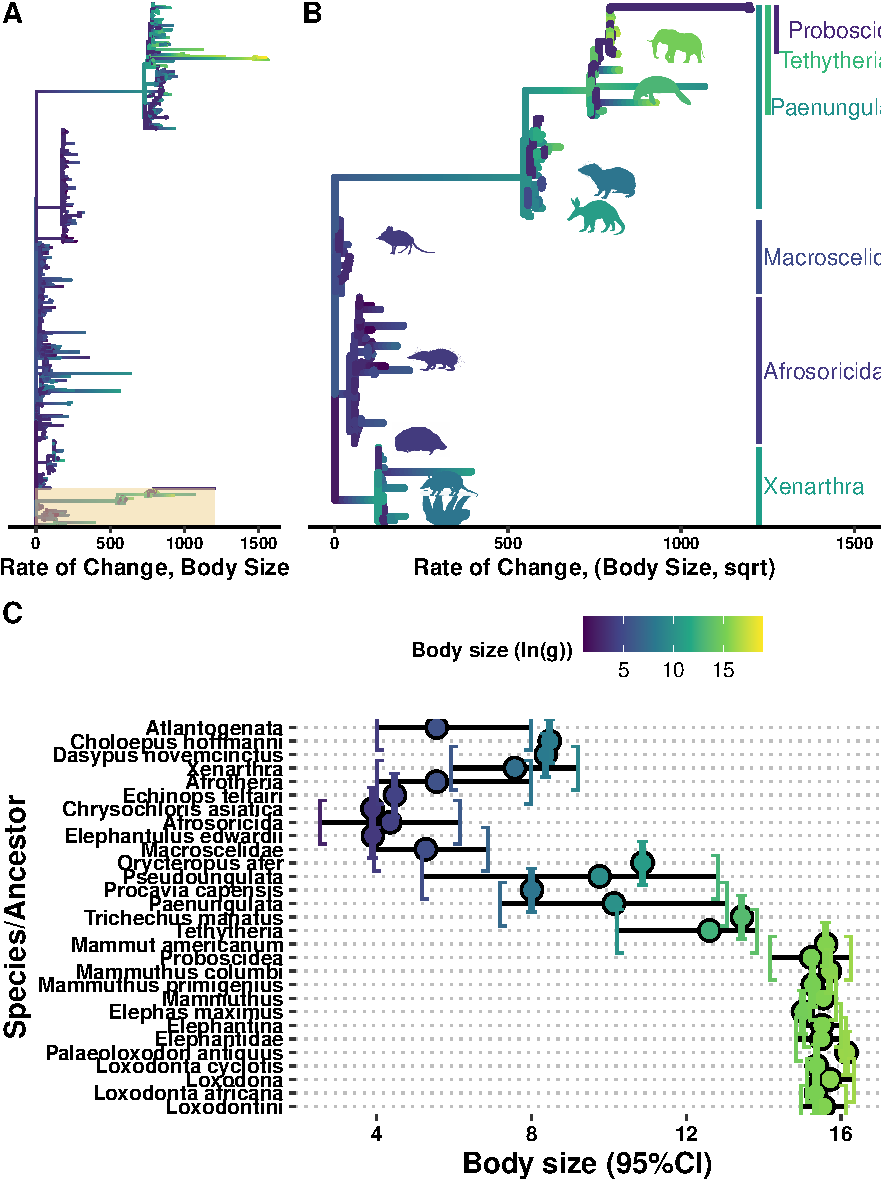
\includegraphics{paper_PLOS_draft_files/figure-latex/Figure 1-1}
\hfill{}

\textbackslash{}caption\{Figure 1: Body sizes rapidly and frequently
expand in Eutherians, especially in Atlantogenata. \textbf{A)} Tree of
Eutherian species, colored by ln(Body Size) and with branch lengths set
to the rate of change in body sizes, normalized by the square root of
the root branch. Atlantogenata is highlighted at the bottom. \textbf{B)}
Zoom-in of (A) on Atlantogenata. Silhuetes for the African Elephant,
West Indian Manatee, Cape Elephant Shrew, Lesser Hedgehog Tenrec, Cape
Golden Mole, Nine-Banded Armadillo, and Hoffman's Two-Toed Sloth are
colored by their extant body sizes, while clade labels are colored based
on the common ancestor's estimated body size\}\label{fig:Figure 1}
\textbackslash{}end\{figure\}

\begin{longtable}[]{@{}lrrrr@{}}
\caption{A table generated by the longtable package.}\tabularnewline
\toprule
Node & Size (log(g)) & 95\% CI (Low) & 95\% CI (High) & Rate
(sqrt)\tabularnewline
\midrule
\endfirsthead
\toprule
Node & Size (log(g)) & 95\% CI (Low) & 95\% CI (High) & Rate
(sqrt)\tabularnewline
\midrule
\endhead
Cryptochloris wintoni & 3.13 & 3.13 & 3.13 & 5.78\tabularnewline
Amblysomus marleyi & 3.53 & 3.53 & 3.53 & 3.79\tabularnewline
Elephantulus revoili & 3.48 & 3.48 & 3.48 & 1.10\tabularnewline
Titanohyrax andrewsi & 12.97 & 12.97 & 12.97 & 0.07\tabularnewline
Titanohyrax ultimus & 14.08 & 14.08 & 14.08 & 34.61\tabularnewline
Megalohyrax sp nov & 12.52 & 12.52 & 12.52 & 7.21\tabularnewline
Elephas maximus asurus & 15.66 & 15.66 & 15.66 & 0.34\tabularnewline
Protenrec tricuspis & 1.14 & 1.14 & 1.14 & 69.75\tabularnewline
Microgale parvula & 1.16 & 1.16 & 1.16 & 33.46\tabularnewline
Microgale pusilla & 1.25 & 1.25 & 1.25 & 34.31\tabularnewline
Geogale aurita & 1.90 & 1.90 & 1.90 & 40.07\tabularnewline
Microgale longicaudata & 2.09 & 2.09 & 2.09 & 0.77\tabularnewline
Microgale brevicaudata & 2.19 & 2.19 & 2.19 & 0.60\tabularnewline
Microgale jobihely & 2.30 & 2.30 & 2.30 & 1.07\tabularnewline
Microgale principula & 2.32 & 2.32 & 2.32 & 0.17\tabularnewline
Dilambdogale gheerbranti & 2.38 & 2.38 & 2.38 & 2.21\tabularnewline
Microgale taiva & 2.47 & 2.47 & 2.47 & 0.13\tabularnewline
Microgale cowani & 2.62 & 2.62 & 2.62 & 0.57\tabularnewline
Eremitalpa granti & 3.14 & 3.14 & 3.14 & 9.65\tabularnewline
Calcochloris obtusirostris & 3.27 & 3.27 & 3.27 & 13.38\tabularnewline
Neamblysomus julianae & 3.33 & 3.33 & 3.33 & 5.72\tabularnewline
Chlorotalpa duthieae & 3.38 & 3.38 & 3.38 & 0.32\tabularnewline
Chlorotalpa sclateri & 3.54 & 3.54 & 3.54 & 0.09\tabularnewline
Macroscelides proboscideus & 3.64 & 3.64 & 3.64 & 14.17\tabularnewline
Chrysochloris stuhlmanni & 3.74 & 3.74 & 3.74 & 0.33\tabularnewline
Oryzorictes hova & 3.79 & 3.79 & 3.79 & 22.77\tabularnewline
Elephantulus myurus & 3.81 & 3.81 & 3.81 & 0.95\tabularnewline
Elephantulus brachyrhynchus & 3.81 & 3.81 & 3.81 & 0.93\tabularnewline
Elephantulus rozeti & 3.81 & 3.81 & 3.81 & 10.51\tabularnewline
Elephantulus fuscus & 3.82 & 3.82 & 3.82 & 0.68\tabularnewline
Elephantulus intufi & 3.82 & 3.82 & 3.82 & 1.15\tabularnewline
Microgale talazaci & 3.88 & 3.88 & 3.88 & 61.40\tabularnewline
Chrysochloris asiatica & 3.89 & 3.89 & 3.89 & 3.34\tabularnewline
Elephantulus edwardii & 3.90 & 3.90 & 3.90 & 0.24\tabularnewline
Carpitalpa arendsi & 3.94 & 3.94 & 3.94 & 0.45\tabularnewline
Amblysomus corriae & 3.94 & 3.94 & 3.94 & 0.98\tabularnewline
Amblysomus hottentotus & 3.98 & 3.98 & 3.98 & 0.02\tabularnewline
Elephantulus fuscipes & 4.04 & 4.04 & 4.04 & 1.93\tabularnewline
Elephantulus rufescens & 4.05 & 4.05 & 4.05 & 0.12\tabularnewline
Neamblysomus gunningi & 4.09 & 4.09 & 4.09 & 3.26\tabularnewline
Elephantulus rupestris & 4.12 & 4.12 & 4.12 & 0.32\tabularnewline
Amblysomus septentrionalis & 4.23 & 4.23 & 4.23 & 0.52\tabularnewline
Chambius kasserinensis & 4.27 & 4.27 & 4.27 & 11.84\tabularnewline
Amblysomus robustus & 4.33 & 4.33 & 4.33 & 1.38\tabularnewline
Micropotamogale lamottei & 4.36 & 4.36 & 4.36 & 2.82\tabularnewline
Echinops telfairi & 4.47 & 4.47 & 4.47 & 7.75\tabularnewline
Limnogale mergulus & 4.52 & 4.52 & 4.52 & 121.95\tabularnewline
Hemicentetes semispinosus & 4.75 & 4.75 & 4.75 & 4.68\tabularnewline
Chrysospalax villosus & 4.77 & 4.77 & 4.77 & 0.13\tabularnewline
Petrodromus tetradactylus & 5.29 & 5.29 & 5.29 & 24.61\tabularnewline
Herodotius pattersoni & 5.50 & 5.50 & 5.50 & 11.64\tabularnewline
Setifer setosus & 5.61 & 5.61 & 5.61 & 12.52\tabularnewline
Rhynchocyon cirnei & 5.86 & 5.86 & 5.86 & 3.30\tabularnewline
Metoldobotes sp nov & 5.93 & 5.93 & 5.93 & 15.94\tabularnewline
Chrysospalax trevelyani & 6.13 & 6.13 & 6.13 & 62.84\tabularnewline
Rhynchocyon petersi & 6.15 & 6.15 & 6.15 & 2.13\tabularnewline
Rhynchocyon chrysopygus & 6.28 & 6.28 & 6.28 & 0.40\tabularnewline
Potamogale velox & 6.49 & 6.49 & 6.49 & 103.04\tabularnewline
Rhynchocyon udzungwensis & 6.57 & 6.57 & 6.57 & 4.33\tabularnewline
Tenrec ecaudatus & 6.75 & 6.75 & 6.75 & 79.50\tabularnewline
Dasypus sabanicola & 7.05 & 7.05 & 7.05 & 12.18\tabularnewline
Tolypeutes matacus & 7.11 & 7.11 & 7.11 & 15.96\tabularnewline
Dasypus septemcinctus & 7.30 & 7.30 & 7.30 & 4.44\tabularnewline
Zaedyus pichiy & 7.31 & 7.31 & 7.31 & 5.54\tabularnewline
Dasypus hybridus & 7.31 & 7.31 & 7.31 & 4.05\tabularnewline
Chaetophractus villosus & 7.61 & 7.61 & 7.61 & 0.42\tabularnewline
Chaetophractus nationi & 7.67 & 7.67 & 7.67 & 0.09\tabularnewline
Heterohyrax brucei & 7.78 & 7.78 & 7.78 & 1.64\tabularnewline
Cabassous centralis & 7.92 & 7.92 & 7.92 & 0.25\tabularnewline
Seggeurius amourensis & 7.98 & 7.98 & 7.98 & 2.82\tabularnewline
Procavia capensis & 8.01 & 8.01 & 8.01 & 0.00\tabularnewline
Dendrohyrax dorsalis & 8.06 & 8.06 & 8.06 & 1.86\tabularnewline
Microhyrax lavocati & 8.13 & 8.13 & 8.13 & 0.73\tabularnewline
Bradypus tridactylus & 8.23 & 8.23 & 8.23 & 0.48\tabularnewline
Bradypus torquatus & 8.27 & 8.27 & 8.27 & 0.03\tabularnewline
Dasypus novemcinctus & 8.37 & 8.37 & 8.37 & 14.73\tabularnewline
Euphractus sexcinctus & 8.43 & 8.43 & 8.43 & 14.99\tabularnewline
Choloepus hoffmanni & 8.47 & 8.47 & 8.47 & 0.32\tabularnewline
Bradypus variegatus & 8.49 & 8.49 & 8.49 & 0.51\tabularnewline
Tamandua tetradactyla & 8.52 & 8.52 & 8.52 & 10.44\tabularnewline
Cyclopes didactylus & 8.53 & 8.53 & 8.53 & 2.15\tabularnewline
Choloepus didactylus & 8.71 & 8.71 & 8.71 & 0.64\tabularnewline
Thyrohyrax meyeri & 8.78 & 8.78 & 8.78 & 3.55\tabularnewline
Saghatherium bowni & 9.13 & 9.13 & 9.13 & 15.85\tabularnewline
Dasypus kappleri & 9.23 & 9.23 & 9.23 & 74.13\tabularnewline
Thyrohyrax domorictus & 9.30 & 9.30 & 9.30 & 1.15\tabularnewline
Dimaitherium patnaiki & 9.57 & 9.57 & 9.57 & 18.23\tabularnewline
Phosphatherium escuilliei & 9.62 & 9.62 & 9.62 & 326.23\tabularnewline
Saghatherium antiquum & 9.73 & 9.73 & 9.73 & 2.90\tabularnewline
Thyrohyrax litholagus & 10.01 & 10.01 & 10.01 & 28.58\tabularnewline
Myrmecophaga tridactyla & 10.26 & 10.26 & 10.26 & 41.03\tabularnewline
Myorycteropus africanus & 10.27 & 10.27 & 10.27 & 0.57\tabularnewline
Selenohyrax chatrathi & 10.73 & 10.73 & 10.73 & 14.99\tabularnewline
Priodontes maximus & 10.82 & 10.82 & 10.82 & 268.43\tabularnewline
Orycteropus afer & 10.87 & 10.87 & 10.87 & 6.59\tabularnewline
Antilohyrax pectidens & 10.93 & 10.93 & 10.93 & 13.69\tabularnewline
Bunohyrax fajumensis & 11.32 & 11.32 & 11.32 & 1.45\tabularnewline
Afrohyrax championi & 11.32 & 11.32 & 11.32 & 0.19\tabularnewline
Geniohyus mirus & 11.33 & 11.33 & 11.33 & 5.44\tabularnewline
Prorastomus sirenoides & 11.49 & 11.49 & 11.49 & 13.61\tabularnewline
Elephas antiquus falconeri & 11.51 & 11.51 & 11.51 & 6.12\tabularnewline
Pachyhyrax crassidentatus & 11.81 & 11.81 & 11.81 & 2.29\tabularnewline
Megalohyrax eocaenus & 11.95 & 11.95 & 11.95 & 0.24\tabularnewline
Elephas cypriotes & 12.21 & 12.21 & 12.21 & 1.90\tabularnewline
Bunohyrax major & 12.36 & 12.36 & 12.36 & 11.39\tabularnewline
Titanohyrax angustidens & 12.48 & 12.48 & 12.48 & 0.04\tabularnewline
Daouitherium rebouli & 12.80 & 12.80 & 12.80 & 0.74\tabularnewline
Arcanotherium savagei & 12.89 & 12.89 & 12.89 & 7.29\tabularnewline
Dugong dugon & 12.92 & 12.92 & 12.92 & 5.85\tabularnewline
Trichechus senegalensis & 13.03 & 13.03 & 13.03 & 0.57\tabularnewline
Trichechus inunguis & 13.08 & 13.08 & 13.08 & 0.69\tabularnewline
Protosiren smithae & 13.20 & 13.20 & 13.20 & 33.69\tabularnewline
Numidotherium koholense & 13.23 & 13.23 & 13.23 & 2.29\tabularnewline
Omanitherium dhofarensis & 13.35 & 13.35 & 13.35 & 0.03\tabularnewline
Trichechus manatus & 13.44 & 13.44 & 13.44 & 1.39\tabularnewline
Moeritherium spp & 13.82 & 13.82 & 13.82 & 5.71\tabularnewline
Phiomia spp & 13.89 & 13.89 & 13.89 & 3.64\tabularnewline
Elephas maximus & 15.02 & 15.02 & 15.02 & 5.81\tabularnewline
Barytherium spp & 15.20 & 15.20 & 15.20 & 73.58\tabularnewline
Mammuthus primigenius & 15.27 & 15.27 & 15.27 & 2.17\tabularnewline
Mammut borsoni & 16.49 & 16.49 & 16.49 & 15.33\tabularnewline
Mammuthus trogontherii & 16.38 & 16.38 & 16.38 & 16.00\tabularnewline
Loxodonta africana & 15.35 & 15.35 & 15.35 & 1.28\tabularnewline
Loxodonta cyclotis & 15.37 & 15.37 & 15.37 & 3.72\tabularnewline
Palaeoloxodon antiquus & 16.14 & 16.14 & 16.14 & 0.01\tabularnewline
Palaeoloxodon namadicus & 16.81 & 16.81 & 16.81 & 12.81\tabularnewline
Mammut americanum & 15.61 & 15.61 & 15.61 & 0.95\tabularnewline
Mammuthus columbi & 15.71 & 15.71 & 15.71 & 0.91\tabularnewline
Hydrodamalis gigas & 15.72 & 15.72 & 15.72 & 172.52\tabularnewline
Atlantogenata & 5.55 & 4.06 & 7.95 & 0.03\tabularnewline
Afrotheria & 5.55 & 4.05 & 7.96 & 0.00\tabularnewline
Afrosorcida & 4.35 & 2.58 & 6.13 & 44.49\tabularnewline
Macroscelidae & 5.27 & 3.98 & 6.85 & 2.49\tabularnewline
Pseudoungulata & 9.76 & 5.21 & 12.78 & 545.83\tabularnewline
Paenungulata & 10.13 & 7.24 & 13.02 & 4.42\tabularnewline
Tethytheria & 12.60 & 10.25 & 13.81 & 187.47\tabularnewline
Proboscidae & 15.23 & 14.22 & 16.24 & 30.28\tabularnewline
Elephantidae & 15.49 & 14.89 & 16.10 & 2.21\tabularnewline
Elephantina & 15.51 & 15.08 & 15.96 & 0.01\tabularnewline
Mammuthus & 15.54 & 15.24 & 15.85 & 0.47\tabularnewline
Loxodontini & 15.55 & 15.02 & 16.11 & 0.11\tabularnewline
Loxodona & 15.72 & 15.16 & 16.30 & 0.86\tabularnewline
Xenarthra & 7.57 & 5.96 & 9.18 & 124.94\tabularnewline
\bottomrule
\end{longtable}

To trace the evolutionary history of body mass and lifespan in
Afrotherians, we built a time-calibrated supertree of Eutherian mammals
combining 1,679 species from Bininda-Emonds et al {[}24{]} with a total
evidence Afrotherian phylogeny including 77 extant and fossil data from
39 extinct species {[}19{]}. Fossil data from extinct species were
included to ensure that ancestral state reconstructions of body mass in
Afrotherians were not biased by only including extant species, which can
lead to inaccurate reconstructions, for example, if lineages multiple
lineages evolved large body masses from a small bodied ancestor. We
jointly estimated rates of body mass evolution and reconstructed
ancestral states using a generalization of a Brownian model of character
evolution, which allows for occasional large jumps in traits (stable
model) and out performs standard Brownian motion and Ornstein-Uhlenbeck
models of character evolution {[}25{]}.

Similar to previous studies of Afrotherian body size {[}19,25{]}, we
found that the body mass of the Afrotherian ancestor was inferred to be
small (0.26kg, 95\% CI: 0.31-3.01kg) and that substantial accelerations
in the rate of body mass evolution occurred coincident with a 2.77x
increase \textbf{(Vinnie wrote 65× increase")} in body mass in the
stem-lineage of \emph{Pseudoungulata} (9.76kg) \textbf{(``Vinnie wrote
(17kg)'')}, a 1.57x increase \textbf{(``Vinnie wrote 1.5x increase'')}
in body mass in the stem-lineage of \emph{Paenungulata} (10.13kg)
\textbf{(``Vinnie wrote (25kg)'')}, a 1.52x increase \textbf{(``Vinnie
wrote 12× increase'')} in body mass in the stem-lineage of
\emph{Tehthytheria} (12.6kg) \textbf{(``Vinnie wrote (296kg)'')}, and a
1.22x increase \textbf{(``Vinnie wrote 14× increase'')} in body mass in
the stem-lineage of \emph{Proboscidea} (15.23kg) \textbf{(``Vinnie wrote
(4,100kg)'')} (Figure 1). The ancestral \emph{Hyracoidea} was inferred
to be relatively small 7.96kg-11.68kg \textbf{(Vinnie wrote
(2.86-15.71kg))}, and rate accelerations were coincident with
independent body mass increases in large hyraxes such as
\emph{Titanohyrax andrewsi} 12.97kg; 1.33x increase (67× increase in
body mass). While the body mass of the ancestral \emph{Sirenian} was
inferred to be large (61-656kg), a rate acceleration occurred coincident
with a 10× body mass increase in Stellar's sea cow. Rate accelerations
also occurred coincident with 36× body mass reduction in the
stem-lineage of the dwarf elephants \emph{Elephas}
(\emph{Palaeoloxodon}) \emph{falconeri} and \emph{Palaeoloxodon
cypriotes}. These data suggest that gigantism in \emph{Afrotherians}
evolved step-wise, from small to medium bodies in the
\emph{Pseudoungulata} stem-lineage, medium to large bodies in the
\emph{Tehthytherian} stem-lineage and extinct hyraxes, and from large to
exceptionally large bodies independently in the \emph{Proboscidean}
stem-lineage and Stellar's sea cow (Figure 1).

\hypertarget{pervasive-duplication-of-tumor-suppressors-during-the-origins-of-large-bodied-afrotheirans}{%
\subsection*{Pervasive duplication of tumor suppressors during the
origins of large bodied
Afrotheirans}\label{pervasive-duplication-of-tumor-suppressors-during-the-origins-of-large-bodied-afrotheirans}}
\addcontentsline{toc}{subsection}{Pervasive duplication of tumor
suppressors during the origins of large bodied Afrotheirans}

\hypertarget{refs}{}
\leavevmode\hypertarget{ref-Green2011}{}%
1. Green J, Cairns BJ, Casabonne D, Wright FL, Reeves G, Beral V, et al.
Height and cancer incidence in the Million Women Study: prospective
cohort, and meta-analysis of prospective studies of height and total
cancer risk. The Lancet Oncology. 2011;12: 785--794.
doi:\href{https://doi.org/10.1016/s1470-2045(11)70154-1}{10.1016/s1470-2045(11)70154-1}

\leavevmode\hypertarget{ref-Nunney:20181c2}{}%
2. Nunney L. Size matters: height, cell number and a person's risk of
cancer. Proc R Soc B. 2018;285: 20181743.
doi:\href{https://doi.org/10.1098/rspb.2018.1743}{10.1098/rspb.2018.1743}

\leavevmode\hypertarget{ref-Dobson2013}{}%
3. Dobson JM. Breed-predispositions to cancer in pedigree dogs. ISRN
veterinary science. 2013;2013: 941275.
doi:\href{https://doi.org/10.1155/2013/941275}{10.1155/2013/941275}

\leavevmode\hypertarget{ref-CaulinAndMaley2011}{}%
4. Caulin AF, Maley CC. Peto's Paradox: evolution's prescription for
cancer prevention. Trends in ecology \& evolution. 2011;26: 175--82.
doi:\href{https://doi.org/10.1016/j.tree.2011.01.002}{10.1016/j.tree.2011.01.002}

\leavevmode\hypertarget{ref-Leroi2003}{}%
5. Leroi AM, Koufopanou V, Burt A. Cancer selection. Nature Reviews
Cancer. 2003;3: 226--231.
doi:\href{https://doi.org/10.1038/nrc1016}{10.1038/nrc1016}

\leavevmode\hypertarget{ref-Peto1975}{}%
6. Peto R, Roe F, Lee P, Levy L, Clack J. Cancer and ageing in mice and
men. British Journal of Cancer. 1975;32: 411--426.
doi:\href{https://doi.org/10.1038/bjc.1975.242}{10.1038/bjc.1975.242}

\leavevmode\hypertarget{ref-Ashur-Fabian2004}{}%
7. Ashur-Fabian O, Avivi A, Trakhtenbrot L, Adamsky K, Cohen M, Kajakaro
G, et al. Evolution of p53 in hypoxia-stressed Spalax mimics human tumor
mutation. Proceedings of the National Academy of Sciences. 2004;101:
12236--12241.
doi:\href{https://doi.org/10.1073/pnas.0404998101}{10.1073/pnas.0404998101}

\leavevmode\hypertarget{ref-Seluanov2008}{}%
8. Seluanov A, Hine C, Bozzella M, Hall A, Sasahara THC, Ribeiro AACM,
et al. Distinct tumor suppressor mechanisms evolve in rodent species
that differ in size and lifespan. Aging cell. 2008;7: 813--23.
doi:\href{https://doi.org/10.1111/j.1474-9726.2008.00431.x}{10.1111/j.1474-9726.2008.00431.x}

\leavevmode\hypertarget{ref-Gorbunova2012}{}%
9. Gorbunova V, Hine C, Tian X, Ablaeva J, Gudkov AV, Nevo E, et al.
Cancer resistance in the blind mole rat is mediated by concerted
necrotic cell death mechanism. Proceedings of the National Academy of
Sciences of the United States of America. 2012;109: 19392--6.
doi:\href{https://doi.org/10.1073/pnas.1217211109}{10.1073/pnas.1217211109}

\leavevmode\hypertarget{ref-Tian2013}{}%
10. Tian X, Azpurua J, Hine C, Vaidya A, Myakishev-Rempel M, Ablaeva J,
et al. High molecular weight hyaluronan mediates the cancer resistance
of the naked mole-rat. 2013;499.
doi:\href{https://doi.org/10.1038/nature12234}{10.1038/nature12234}

\leavevmode\hypertarget{ref-Sulak2016}{}%
11. Sulak M, Fong L, Mika K, Chigurupati S, Yon L, Mongan NP, et al.
TP53 copy number expansion is associated with the evolution of increased
body size and an enhanced DNA damage response in elephants. eLife.
2016;5: e11994.
doi:\href{https://doi.org/10.7554/elife.11994}{10.7554/elife.11994}

\leavevmode\hypertarget{ref-HAGR}{}%
12. Tacutu R, Craig T, Budovsky A, Wuttke D, Lehmann G, Taranukha D, et
al. Human Ageing Genomic Resources: Integrated databases and tools for
the biology and genetics of ageing. Nucleic Acids Research. 2013;41:
D1027--D1033.
doi:\href{https://doi.org/10.1093/nar/gks1155}{10.1093/nar/gks1155}

\leavevmode\hypertarget{ref-Schwartz1995}{}%
13. Schwartz GT, Rasmussen DT, Smith RJ. Body-Size Diversity and
Community Structure of Fossil Hyracoids. Journal of Mammalogy. 1995;76:
1088--1099. doi:\href{https://doi.org/10.2307/1382601}{10.2307/1382601}

\leavevmode\hypertarget{ref-Scheffer1972}{}%
14. Scheffer VB. The Weight of the Steller Sea Cow. Journal of
Mammalogy. 1972;53: 912--914.
doi:\href{https://doi.org/10.2307/1379236}{10.2307/1379236}

\leavevmode\hypertarget{ref-Larramendi:20151c2}{}%
15. Larramendi A. Shoulder Height, Body Mass, and Shape of
Proboscideans. Acta Palaeontologica Polonica. 2015;61.
doi:\href{https://doi.org/10.4202/app.00136.2014}{10.4202/app.00136.2014}

\leavevmode\hypertarget{ref-OLeary2013a}{}%
16. O'Leary MA, Bloch JI, Flynn JJ, Gaudin TJ, Giallombardo A, Giannini
NP, et al. The placental mammal ancestor and the post-K-Pg radiation of
placentals. Science (New York, NY). 2013;339: 662--7.
doi:\href{https://doi.org/10.1126/science.1229237}{10.1126/science.1229237}

\leavevmode\hypertarget{ref-Springer2013}{}%
17. Springer MS, Meredith RW, Teeling EC, Murphy WJ. Technical comment
on "The placental mammal ancestor and the post-K-Pg radiation of
placentals". Science (New York, NY). 2013;341: 613.
doi:\href{https://doi.org/10.1126/science.1238025}{10.1126/science.1238025}

\leavevmode\hypertarget{ref-OLeary2013b}{}%
18. O'Leary MA, Bloch JI, Flynn JJ, Gaudin TJ, Giallombardo A, Giannini
NP, et al. Response to comment on "The placental mammal ancestor and the
post-K-Pg radiation of placentals". Science (New York, NY). 2013;341:
613.
doi:\href{https://doi.org/10.1126/science.1238162}{10.1126/science.1238162}

\leavevmode\hypertarget{ref-PuttickAndThomas2015}{}%
19. Puttick MN, Thomas GH. Fossils and living taxa agree on patterns of
body mass evolution: a case study with Afrotheria. Proceedings
Biological sciences / The Royal Society. 2015;282: 20152023.
doi:\href{https://doi.org/10.1098/rspb.2015.2023}{10.1098/rspb.2015.2023}

\leavevmode\hypertarget{ref-Abegglen:JAMA2015}{}%
20. Abegglen LM, Caulin AF, Chan A, Lee K, Robinson R, Campbell MS, et
al. Potential Mechanisms for Cancer Resistance in Elephants and
Comparative Cellular Response to DNA Damage in Humans. JAMA. 2015;314:
1850--1860.
doi:\href{https://doi.org/10.1001/jama.2015.13134}{10.1001/jama.2015.13134}

\leavevmode\hypertarget{ref-Vazquez2018}{}%
21. Vazquez JM, Sulak M, Chigurupati S, Lynch VJ. A Zombie LIF Gene in
Elephants Is Upregulated by TP53 to Induce Apoptosis in Response to DNA
Damage. Cell Reports. 2018;24: 1765--1776.
doi:\href{https://doi.org/10.1016/j.celrep.2018.07.042}{10.1016/j.celrep.2018.07.042}

\leavevmode\hypertarget{ref-Caulin2015}{}%
22. Caulin AF, Graham TA, Wang L-S, Maley CC. Solutions to Peto's
paradox revealed by mathematical modelling and cross-species cancer gene
analysis. Philosophical transactions of the Royal Society of London
Series B, Biological sciences. 2015;370: 20140222.
doi:\href{https://doi.org/10.1098/rstb.2014.0222}{10.1098/rstb.2014.0222}

\leavevmode\hypertarget{ref-Doherty2016}{}%
23. Doherty A, Magalhães J de. Has gene duplication impacted the
evolution of Eutherian longevity? Aging Cell. 2016;15: 978--980.
doi:\href{https://doi.org/10.1111/acel.12503}{10.1111/acel.12503}

\leavevmode\hypertarget{ref-Bininda-Emonds2008}{}%
24. Bininda-Emonds ORP, Cardillo M, Jones KE, MacPhee RDE, Beck RMD,
Grenyer R, et al. Erratum: The delayed rise of present-day mammals.
Nature. 2008;456: 274--274.
doi:\href{https://doi.org/10.1038/nature07347}{10.1038/nature07347}

\leavevmode\hypertarget{ref-ElliotAndMooers2014}{}%
25. Elliot MG, Mooers AØ. Inferring ancestral states without assuming
neutrality or gradualism using a stable model of continuous character
evolution. BMC evolutionary biology. 2014;14: 226.
doi:\href{https://doi.org/10.1186/s12862-014-0226-8}{10.1186/s12862-014-0226-8}

\leavevmode\hypertarget{ref-blat}{}%
26. Kent JW. BLAT---The BLAST-Like Alignment Tool. Genome Research.
2002;12: 656--664.
doi:\href{https://doi.org/10.1101/gr.229202}{10.1101/gr.229202}

\leavevmode\hypertarget{ref-AltenhoffAndDessimoz2009}{}%
27. Altenhoff AM, Dessimoz C. Phylogenetic and functional assessment of
orthologs inference projects and methods. PLoS computational biology.
2009;5: e1000262.
doi:\href{https://doi.org/10.1371/journal.pcbi.1000262}{10.1371/journal.pcbi.1000262}

\leavevmode\hypertarget{ref-uniprot}{}%
28. Consortium TU. UniProt: the universal protein knowledgebase. Nucleic
Acids Research. 2017;45: D158--D169.
doi:\href{https://doi.org/10.1093/nar/gkw1099}{10.1093/nar/gkw1099}

\nolinenumbers


\end{document}

